% Volume III, Chapter 3 (drafted as "Chapter 29")
\chapter{Phase Oscillators on Buildings: Chiral Connections, Frustrated Ground States, and Transverse Bifurcations}\label{chap:V3P3}
\chaptermark{Phase Oscillators on Buildings}
\begin{chapterabstract}
The proposed programme asks for a gauge-covariant Kuramoto model on an $\Atwo$ complex, with pairwise
coupling $K_1$ through a connection $A$ of chamber flux $2\pi\alpha_0$ and a triadic chamber
coupling $K_2$ with lag $\Phi$. It then asks for proofs of four claims. (a) The flux breaks
time reversal and forbids static fixed points, forcing a permanent chiral limit cycle. (b) An
Ott--Antonsen reduction closes on the three type classes, and a supercritical Hopf
bifurcation produces a chimera with one class coherent and two incoherent. (c) The Berry phase
of the synchronized cycle is topological. (d) The frequency shift is fixed by the Euler
characteristic and the number of chambers. We prove what is true and correct what is not.

(1) \emph{Chiral connections.} The uniform connection $A^{\alpha}=\frac{2\pi\alpha}{3}\mathbf
1_E$ has flux $2\pi\alpha$ on every chamber of every $\Atwo$ complex. Chiral connections of a
given flux form a torsor under $\Hom(H_1(Y;\Z),U(1))$, which is finite on thick complexes by
Garland rigidity ($64$ classes on $Y_{21}$). The triadic lag $\Phi$ is \emph{not} a gauge
field: the only gauge-covariant triadic term is blind to the flux.

(2) \emph{The flux sector is a gradient flow.} For $K_2=0$ and identical frequencies, the
model is the gradient flow of a frustrated XY energy for every flux. Every trajectory
converges to an equilibrium, all Jacobians are symmetric, and there are no limit cycles and
no Hopf bifurcations. Claim (a) is therefore false. The ground states are the three
\emph{twisted states} $\theta_j=\frac{2\pi m}{3}\tau(j)$; we determine exactly which of them
minimize the energy. The flux produces static persistent currents, not rotation.

(3) \emph{The triadic lag.} For all parameters the twisted states are relative equilibria
rotating at $\Omega=\omega+K_2\sin\Phi$. Their Jacobian is $-c_m\Delta_0$, so its spectrum is
real, stability changes only through a real, $(n-1)$-fold degenerate crossing, and never
through a Hopf bifurcation. On the type-cluster subspace the whole system is a gradient flow
modulo rotation. At every cluster equilibrium the Jacobian splits into $3\times3$ blocks
$M(\lambda)$ indexed by the $\Z/3$-orbits of eigenvalues of $A_1$. On $Y_{21}$ every block is
real. On $Y_{168}$ a stable cluster state can lose stability through a complex pair of a transverse
block; this happens at about a fifth of the losses of stability found, always with multiplicity $21$,
and in every case examined the network then freezes into a locked state instead of a limit cycle.

(4) \emph{Ott--Antonsen and chimeras.} The OA manifold is invariant only for $K_2=0$: the
triadic term is second harmonic in $\theta_j$, and we prove non-closure. For $K_2=0$ we derive
the closed equations for $(r_t,\psi_t)$ and a Lyapunov function that excludes chimeras and
Hopf bifurcations for identical oscillators. For $K_2\ne0$ the chimera of (b) remains
unproved. Numerically it is never the primary instability of a stable cluster state, and it
did not appear in our runs.

(5) \emph{Phases and frequencies.} A rigid rotation has zero geometric phase. The genuine
geometric datum is the monodromy of the twisted states under threading one flux quantum per
chamber. It is the cyclic permutation $\Theta_m\mapsto\Theta_{m+1}$, implemented by the
grading character of Chapter~\ref{chap:V3P1}. The frequency shift is $K_2\langle m_\Delta\rangle_F$, a local
quantity. The identity $D_2=3|F|/\chi(Y)$ holds only for $q=2$; on the thin torus $\chi=0$
while the shift is not. Trees fail for two reasons: every connection on a tree is pure gauge,
and without $2$-cells the dynamics is a gradient flow.
\end{chapterabstract}

\section*{Status of the results}

Every numbered statement is proved. The exceptions are the numerical observations in
Remark~\ref{V3P3:rem:numerics}, Theorem~\ref{V3P3:thm:hopf} and Remark~\ref{V3P3:rem:hopfdyn}, which
are numerical, and two classical inputs: the \L{}ojasiewicz convergence
theorem for analytic gradient flows \cite{Loj63} and LaSalle's invariance principle
\cite{LaSalle60}. The Ott--Antonsen equations are derived here in the form used, together with
their failure for $K_2\ne0$. All finite identities, and the numerical statements, were checked
by \texttt{code/v3p3\_verify.py} (Table~\ref{V3P3:tab:battery}).

Notation follows Chapters~\ref{chap:V3P1}--\ref{chap:V3P2}. $Y$ is a finite $\Atwo$ complex satisfying (L) for some
$q\ge1$. For $q=1$ this means the thin tori, whose links are hexagons. Put
$\kappa=q^{2}+q+1$. Then every vertex has $\kappa$ out-neighbours (type $+1$) and $\kappa$
in-neighbours (type $-1$), every edge lies in $q+1$ chambers, every vertex lies in
$D_2=\kappa(q+1)$ chambers, and $|E|=\kappa n$, $3|F|=nD_2$. Edges are oriented
$j\to k$ with $\tau(k)=\tau(j)+1$, chambers are oriented $a\to b\to c\to a$, and
$P_t$ is the projection onto the class $V_t=\tau^{-1}(t)$, of size $n/3$. As in Vol.~I--II,
Definition~\ref{M-X:def:a2}, $A_1$ is normal: $A_1A_1^{t}=A_1^{t}A_1$.

\section{The model and its gauge structure}\label{V3P3:sec:model}

\begin{definition}[Connections and flux]\label{V3P3:def:conn}
A \emph{connection} is a function $A$ on ordered adjacent pairs with $A_{kj}=-A_{jk}$, taken
modulo $2\pi$. Equivalently, it is a $1$-cochain $A\in C^{1}(Y;\R/2\pi\Z)$ on the oriented
edges. Its \emph{flux} is the $2$-cochain $\delta A$, with
$(\delta A)(a,b,c)=A_{ab}+A_{bc}+A_{ca}$. $A$ is \emph{chiral of flux $2\pi\alpha$} if
$\delta A=2\pi\alpha$ on every (type-increasingly oriented) chamber. A \emph{gauge
transformation} $\chi\in C^{0}(Y;\R)$ acts by $\theta_j\mapsto\theta_j+\chi_j$,
$A_{jk}\mapsto A_{jk}-(\chi_k-\chi_j)$. It preserves the link variables
$\varphi_{jk}=\theta_k-\theta_j+A_{jk}$ and the flux.
\end{definition}

\begin{proposition}[Chiral connections]\label{V3P3:prop:chiral}
\begin{enumerate}
\item[(i)] For every $\alpha\in\R$ the uniform connection $A^{\alpha}$, equal to
$a=\frac{2\pi\alpha}{3}$ on every oriented edge, is chiral of flux $2\pi\alpha$.
\item[(ii)] $A^{\alpha+1}$ is gauge equivalent to $A^{\alpha}$, via the type gauge
$\chi=\frac{2\pi}{3}\tau$. In particular $A^{m}$ is pure gauge for $m\in\Z$.
\item[(iii)] The gauge classes of chiral connections of flux $2\pi\alpha$ form a torsor under
$\Hom(H_1(Y;\Z),U(1))$. If $q\ge2$, this group is finite of order $|H_1(Y;\Z)|$
(Theorem~\ref{V3P1:thm:garland}). On $Y_{21}$, where $H_1=(\Z/2)^{6}$, there are $64$ classes.
\end{enumerate}
\end{proposition}

\begin{proof}
(i) Each chamber has three oriented edges. (ii) $\chi_k-\chi_j=\frac{2\pi}{3}$ on every edge
$j\to k$. (iii) If $A,A'$ are both chiral of flux $2\pi\alpha$, then $\delta(A-A')=0$, so
$A-A'$ is a flat connection. Modulo gauge, flat connections form $H^{1}(Y;\R/2\pi\Z)$, which
equals $\Hom(H_1(Y;\Z),\R/2\pi\Z)$ by the universal coefficient theorem, because $\R/2\pi\Z$ is
divisible. When $b_1=0$ this is the Pontryagin dual of the finite group $H_1$.
\end{proof}

So the constant flux imposes no quantization. The $2$-cochain $\mathbf 1_F=\frac13\delta\mathbf
1_E$ is exact, and every integral $2$-cycle has zero chamber sum.

\begin{definition}[The model]\label{V3P3:def:model}
For $\omega\in\R$, $K_1,K_2\in\R$, $\alpha,\Phi\in\R$ and $a=\frac{2\pi\alpha}{3}$:
\begin{equation}\label{V3P3:eq:model}
\dot\theta_j=\omega_j+\frac{K_1}{2\kappa}\sum_{k\sim j}\sin(\theta_k-\theta_j+A^{\alpha}_{jk})
+\frac{K_2}{D_2}\sum_{\{j,k,l\}\in F}\sin(\theta_k+\theta_l-2\theta_j+\Phi).
\end{equation}
Unless stated otherwise, $\omega_j=\omega$ for all $j$. Write $\varphi_e$ for the link variable on a
type-increasing edge $e$, and for a chamber $\Delta$ with corner $j$ write
$x^{\Delta}_j=\theta_k+\theta_l-2\theta_j$ and $m_\Delta=\frac13\sum_{j\in\Delta}
\sin(x^{\Delta}_j+\Phi)$.
\end{definition}

\begin{remark}[The triadic lag is not a gauge field]\label{V3P3:rem:lag}
The pairwise term of \eqref{V3P3:eq:model} is gauge covariant, but the triadic term with a
corner-independent $\Phi$ is not: under $\chi$ its argument shifts by
$\chi_k+\chi_l-2\chi_j$. The covariant triadic term built from the connection is
$\sin(\varphi_{jk}+\varphi_{jl})$. Its three corner arguments sum to
$\sum(\varphi_{jk}+\varphi_{kj})=0$, whatever the flux, and in the gauge $A^{\alpha}$ it
equals the $\Phi=0$ term of \eqref{V3P3:eq:model}, because $A_{jk}+A_{jl}=a-a=0$. Thus the
flux $\alpha$ and the lag $\Phi$ are independent parameters. $\Phi$ is a Sakaguchi-type lag
\cite{SK86} on the triadic coupling of Skardal--Arenas type \cite{SA19}, not a curvature.
\end{remark}

\section{Symmetries and the gradient sector}\label{V3P3:sec:gradient}

The model is invariant under the global rotation $\theta\mapsto\theta+c\mathbf 1$. The
conjugation $C\colon\theta\mapsto-\theta$ maps the parameters $(\omega,\alpha,\Phi)$ to
$(-\omega,-\alpha,-\Phi)$. Since $\alpha$ matters only modulo $1$
(Proposition~\ref{V3P3:prop:chiral}(ii)), the flux is $C$-invariant exactly when
$\alpha\in\frac12\Z$. This is the precise sense in which the flux is ``T-odd''.

\begin{proposition}[Frequency sum rule]\label{V3P3:prop:sum}
For every state $\theta$ and arbitrary $\omega_j$,
\[
\frac1n\sum_j\dot\theta_j=\bar\omega+K_2\,\langle m_\Delta\rangle_F,\qquad
\langle m_\Delta\rangle_F=\frac1{|F|}\sum_{\Delta\in F}m_\Delta .
\]
Hence every frequency-locked state has $|\Omega-\bar\omega|\le|K_2|$, and for $K_2=0$ its
frequency is $\bar\omega$ whatever the flux.
\end{proposition}

\begin{proof}
Each edge contributes $\sin\varphi_e-\sin\varphi_e=0$ to the pairwise part, because all
degrees are equal to $2\kappa$. Each chamber contributes $3m_\Delta$ to the triadic part, and
$nD_2=3|F|$.
\end{proof}

\begin{theorem}[The flux sector is a gradient flow]\label{V3P3:thm:gradient}
Let $G$ be any finite graph and $A$ any connection on it. Suppose $K_2=0$ and
$\omega_j=\omega$. In the frame rotating at $\omega$, the model
$\dot\theta_j=\frac{K_1}{\deg j}\sum_{k\sim j}\sin\varphi_{jk}$ is the gradient flow of
\[
V_A(\theta)=-K_1\sum_{e}\cos\varphi_e
\]
for the metric $\sum_j\deg(j)\,d\theta_j^{2}$. Consequently:
\begin{enumerate}
\item[(i)] every trajectory converges to a single equilibrium;
\item[(ii)] at every equilibrium the Jacobian is self-adjoint for this metric, so its spectrum
is real;
\item[(iii)] there is no periodic orbit other than equilibria, and no Hopf bifurcation, for any
flux.
\end{enumerate}
In particular, in the model \eqref{V3P3:eq:model} with $K_2=0$ a nonzero flux does not
prevent static fixed points and does not force rotation.
\end{theorem}

\begin{proof}
$\partial V_A/\partial\theta_j=-K_1\sum_{k\sim j}\sin\varphi_{jk}$, because
$\varphi_{kj}=-\varphi_{jk}$. So $\dot\theta_j=-\deg(j)^{-1}\partial_jV_A$. $V_A$ is real
analytic on the compact torus, so by \L{}ojasiewicz \cite{Loj63} every trajectory has finite
length and converges. The Jacobian is $-g^{-1}\operatorname{Hess}V_A$, which is self-adjoint
for $g$. Along a non-constant orbit $V_A$ strictly decreases, which excludes periodic orbits.
\end{proof}

\begin{lemma}[Triangle lemma]\label{V3P3:lem:triangle}
Let $S\in[-\pi,\pi]$. On $\{x\in\R^{3}:x_1+x_2+x_3\equiv S\bmod2\pi\}$,
$\max\sum_i\cos x_i=3\cos(S/3)$. For $|S|<\pi$ the maximum is attained only at
$x_i\equiv S/3$.
\end{lemma}

\begin{proof}
At a critical point the Lagrange condition gives $\sin x_1=\sin x_2=\sin x_3$, so each
$x_i\in\{u,\pi-u\}$ modulo $2\pi$. If all three equal $u$ (or all equal $\pi-u$), the value is
$3\cos\frac{S+2\pi k}{3}$ for some $k$, and it is largest for $k=0$ because $|S|\le\pi$. If the
two values are mixed, then either $(u,u,\pi-u)$ with $u\equiv S-\pi$, of value $\cos u$, or
$(u,\pi-u,\pi-u)$ with $u\equiv-S$, of value $-\cos u$; both equal $-\cos S$. Put
$c=S/3\in[-\frac\pi3,\frac\pi3]$. Then
$3\cos c-(-\cos3c)=4\cos^{3}c>0$.
\end{proof}

\begin{theorem}[Frustrated ground states]\label{V3P3:thm:ground}
Let $K_1>0$ and $K_2=0$. Write $\alpha=\operatorname{round}(\alpha)+\beta$ with
$\beta\in[-\frac12,\frac12]$, and define the \emph{twisted states}
$\Theta_m=\frac{2\pi m}{3}\tau$, $m\in\Z/3$. Then
\[
\min V_{A^{\alpha}}=-K_1|E|\cos\tfrac{2\pi\beta}{3}.
\]
The minimizers are the rotations of $\Theta_{m_*}$, $m_*\equiv-\operatorname{round}(\alpha)$.
At a minimizer every type-increasing edge carries the same link variable $\frac{2\pi\beta}{3}$,
and hence the static current $K_1\sin\frac{2\pi\beta}3$. For $|\beta|<\frac12$ the minimizer
is unique up to rotation. For $\alpha\in\frac12+\Z$ there are exactly two minimizers, with link
variables $\pm\frac\pi3$, and $C$ exchanges them.
\end{theorem}

\begin{proof}
Around each chamber $\varphi_{ab}+\varphi_{bc}+\varphi_{ca}=3a=2\pi\alpha\equiv2\pi\beta$,
because the $\theta$-differences cancel. Each edge lies in $q+1$ chambers, so by
Lemma~\ref{V3P3:lem:triangle}
\[
\sum_e\cos\varphi_e=\frac1{q+1}\sum_{\Delta}\sum_{e\subset\Delta}\cos\varphi_e
\le\frac{3|F|}{q+1}\cos\tfrac{2\pi\beta}3=|E|\cos\tfrac{2\pi\beta}3 .
\]
On $\Theta_m$ every link variable is $\frac{2\pi(m+\alpha)}{3}$, which gives equality for
$m=m_*$. If $|\beta|<\frac12$, equality forces $\varphi_e\equiv\frac{2\pi\beta}3$ on every
edge. Then $\theta_k-\theta_j\equiv\frac{2\pi m_*}{3}$ along every edge $j\to k$, so $\theta$ is
a rotation of $\Theta_{m_*}$ ($Y$ is connected). At $|\beta|=\frac12$, equality forces each
chamber to carry $\frac\pi3$ on all three edges or $-\frac\pi3$ on all three. Two chambers
sharing an edge agree. $Y$ is gallery connected, because it is connected and its links are
connected. So the value is the same everywhere, and $\theta$ is a rotation of one of the two
twisted states with link variables $\pm\frac\pi3$. $C$ reverses link variables, so it exchanges
them.
\end{proof}

\section{Twisted states and the triadic lag}\label{V3P3:sec:twisted}

\begin{theorem}[Twisted states for all parameters]\label{V3P3:thm:twisted}
For all $K_1,K_2,\alpha,\Phi$ and $m\in\Z/3$, the state $\Theta_m+\Omega t$ with
$\Omega=\omega+K_2\sin\Phi$ is a solution of \eqref{V3P3:eq:model}. The Jacobian at $\Theta_m$ is
\[
J_m=-c_m\,\Delta_0,\qquad
c_m=\frac{K_1\cos\frac{2\pi(m+\alpha)}3+2K_2\cos\Phi}{2\kappa}.
\]
Its eigenvalues are $-c_m\lambda_i(\Delta_0)$. $\Theta_m$ is linearly stable modulo rotation
if and only if $c_m>0$. When $c_m$ changes sign, all $n-1$ transverse eigenvalues cross zero
together, along the real axis. In particular no Hopf bifurcation ever occurs at a twisted
state.
\end{theorem}

\begin{proof}
On $\Theta_m$ every link variable is $\pm\frac{2\pi(m+\alpha)}{3}$, and the pairwise
contributions from out- and in-neighbours cancel. Every triadic argument is
$\frac{2\pi m}{3}(\tau_k+\tau_l-2\tau_j)+\Phi=2\pi m+\Phi$. Differentiating the pairwise term
gives $-\frac{K_1}{2\kappa}\cos\frac{2\pi(m+\alpha)}{3}\Delta_0$. For the triadic term,
$\partial_{\theta_k}$ of the $j$-th equation is $\frac{K_2}{D_2}\cos\Phi$ times the number
$q+1$ of chambers containing $j$ and $k$, and $\partial_{\theta_j}$ is $-2K_2\cos\Phi$. Since
$D_2=\kappa(q+1)$, the triadic part is $\frac{K_2\cos\Phi}{\kappa}(A_1+A_2-2\kappa
I)=-\frac{K_2\cos\Phi}{\kappa}\Delta_0$.
\end{proof}

\begin{corollary}[Multistability]\label{V3P3:cor:bistable}
Let $K_2=0$ and $K_1>0$. $\Theta_m$ is stable iff the distance from $m+\alpha$ to $3\Z$ is less
than $\frac34$. Two twisted states are stable exactly when the fractional part of $\alpha$
lies in $(\frac14,\frac34)$, and otherwise only the ground state is. Varying $\alpha$ therefore
produces hysteresis.
\end{corollary}

\paragraph{The type-cluster subspace.} If $\omega_j=\omega$, the subspace
$\{\theta_j=\psi_{\tau(j)}\}$ is invariant: a vertex of type $t$ sees $\kappa$ neighbours of
types $t\pm1$, and each of its chambers has one vertex of each type. With
$d_t=\psi_{t+1}-\psi_t$ (indices mod $3$) the reduced equations are
\begin{equation}\label{V3P3:eq:cluster}
\dot\psi_t=\omega+\tfrac{K_1}{2}\bigl[\sin(d_t+a)-\sin(d_{t-1}+a)\bigr]+K_2\sin(d_t-d_{t-1}+\Phi).
\end{equation}

\begin{theorem}[Gradient structure modulo rotation]\label{V3P3:thm:clustergrad}
Put $U(\psi)=-\frac{K_1}2\sum_t\cos(d_t+a)-\frac{K_2}3\sum_t\cos(d_t-d_{t-1}+\Phi)$. Then
\eqref{V3P3:eq:cluster} reads
$\dot\psi=\omega\mathbf 1-\nabla U+\bar m(\psi)\mathbf 1$ with
$\bar m=\frac{K_2}3\sum_t\sin(d_t-d_{t-1}+\Phi)$. Modulo rotation it is therefore the
gradient flow of $U$. Every cluster trajectory converges to a relative equilibrium, the reduced
Jacobian is symmetric, and there are no periodic orbits or Hopf bifurcations inside the
cluster subspace. For the full network,
\[
\dot\theta=\omega\mathbf 1-\nabla\Bigl(\tfrac{1}{2\kappa}V_{A^{\alpha}}+\tfrac{K_2}{D_2}
\sum_\Delta W_\Delta\Bigr)+\tfrac{K_2}{D_2}\sum_{\Delta}m_\Delta(\theta)\,\mathbf 1_\Delta ,
\qquad W_\Delta=-\tfrac13\sum_{j\in\Delta}\cos(x^{\Delta}_j+\Phi),
\]
so the only non-gradient part is the \emph{chamber drive} $\sum_\Delta m_\Delta\mathbf
1_\Delta$. It is parallel to $\mathbf 1$ whenever all $m_\Delta$ are equal.
\end{theorem}

\begin{proof}
For one chamber,
$-\partial_{\theta_s}W_\Delta=\sin(x^{\Delta}_s+\Phi)-m_\Delta$, because
$\partial x^{\Delta}_j/\partial\theta_s$ is $-2$ for $j=s$ and $1$ otherwise. Summing over chambers
gives the decomposition. On the cluster subspace all $m_\Delta$ equal $\bar m/K_2$, and
$\sum_\Delta\mathbf 1_\Delta=D_2\mathbf 1$. The reduced flow on $T^{3}/S^{1}$ is then the
gradient of $U$, and the \L{}ojasiewicz argument of Theorem~\ref{V3P3:thm:gradient} applies.
\end{proof}

\begin{theorem}[Block decomposition at cluster equilibria]\label{V3P3:thm:blocks}
Let $\psi$ be an equilibrium of \eqref{V3P3:eq:cluster} and $\theta=\psi\circ\tau$. Put
$p_t=\frac{K_1}{2\kappa}\cos(d_t+a)$ and $c_t=\frac{K_2}{\kappa}\cos(d_t-d_{t-1}+\Phi)$, and
\[
\alpha_t=p_t+c_t,\qquad \gamma_t=p_{t-1}+c_t,\qquad \sigma_t=\kappa(\alpha_t+\gamma_t).
\]
Then $J=-\sum_t\sigma_tP_t+\sum_tP_t(\alpha_tA_1+\gamma_tA_2)$, and
$\C^{n}=W_0\oplus\bigoplus_{[\lambda]}W_{[\lambda]}$ is a $J$-invariant decomposition. Here
$W_0=\ker A_1$, and $W_{[\lambda]}=E_\lambda\oplus E_{\omega\lambda}\oplus
E_{\omega^{2}\lambda}$ runs over the $\Z/3$-orbits of nonzero eigenvalues of $A_1$, with
$\omega=e^{2\pi i/3}$. On $W_0$, $J$ acts as $-\sigma_t$ on $W_0\cap\C^{V_t}$. On
$W_{[\lambda]}$ it acts as $M(\lambda)\otimes I_{\dim E_\lambda}$, where
\[
M(\lambda)=\begin{pmatrix}-\sigma_0&\alpha_0\lambda&\gamma_0\bar\lambda\\
\gamma_1\bar\lambda&-\sigma_1&\alpha_1\lambda\\ \alpha_2\lambda&\gamma_2\bar\lambda&-\sigma_2
\end{pmatrix}.
\]
The orbit of $\lambda=\kappa$ is the tangent space of the cluster subspace, and $M(\kappa)$ is
the Jacobian of \eqref{V3P3:eq:cluster}. The rates $\sigma_t$ are the mean-field transverse
rates of the classes.
\end{theorem}

\begin{proof}
The entries of $J$ follow as in Theorem~\ref{V3P3:thm:twisted}. Row $j\in V_t$ has $\alpha_t$ at
each out-neighbour, $\gamma_t$ at each in-neighbour, and $-\sigma_t$ on the diagonal, because
rows sum to zero. Let $D_1=\operatorname{diag}(\omega^{-\tau})$. Then $D_1A_1D_1^{-1}=\omega
A_1$ (Proposition~\ref{V3P1:prop:grading}), so $D_1$ permutes the eigenspaces within an orbit
and $P_t=\frac13\sum_k\omega^{kt}D_1^{k}$ preserves $W_{[\lambda]}$ and $W_0$. $A_1$ is
normal, so $A_2=A_1^{*}$ acts as $\bar\lambda$ on $E_\lambda$. For $v\in E_\lambda$ we have
$A_1P_sv=P_{s-1}A_1v=\lambda P_{s-1}v$ and $A_2P_sv=\bar\lambda P_{s+1}v$. If $P_sv=0$ for one
$s$, these relations force $v=0$, since $\lambda\neq0$. So $\{P_sv_i\}$, for an orthonormal
basis $(v_i)$ of $E_\lambda$, is a basis of $W_{[\lambda]}$, and
$J(P_sv)=-\sigma_sP_sv+\alpha_{s-1}\lambda P_{s-1}v+\gamma_{s+1}\bar\lambda P_{s+1}v$, which
is the stated matrix. On $W_0$ both $A_1$ and $A_2$ vanish.
\end{proof}

\begin{corollary}\label{V3P3:cor:Y21real}
On $Y_{21}$ the Jacobian at every type-cluster equilibrium has real spectrum. So no Hopf
bifurcation occurs at any cluster state of $Y_{21}$.
\end{corollary}

\begin{proof}
The $1$-skeleton is $K_{7,7,7}$ (Proposition~\ref{V3P2:prop:k777}), so
$A_1=C_3\otimes J_7$, with spectrum $7\{1,\omega,\omega^{2}\}$ and $0^{(18)}$. The only block is
$M(7)$, whose spectrum is that of the reduced cluster Jacobian, and this is real by
Theorem~\ref{V3P3:thm:clustergrad}. The remaining eigenvalues are the real numbers $-\sigma_t$.
\end{proof}

On complexes where $A_1$ has nontrivial eigenvalue orbits, $M(\lambda)$ can have complex
eigenvalues. On $Y_{168}$ this happened at $6$ of the equilibria sampled in line (B) of
Table~\ref{V3P3:tab:battery}. A Hopf bifurcation \emph{transverse} to the cluster subspace is
therefore not excluded in general. Section~\ref{V3P3:sec:hopf} shows that it occurs on $Y_{168}$, with
multiplicity $21$ forced by the symmetry, and that the resulting loss of stability is hard.

\section{Mean field and Ott--Antonsen reduction}\label{V3P3:sec:oa}

Replace neighbour sums by class averages $Z_t=r_te^{i\psi_t}=\frac3n\sum_{j\in
V_t}e^{i\theta_j}$, and the pair sum over chambers by $Z_{t+1}Z_{t-1}$. For $j\in V_t$ this
gives
\begin{equation}\label{V3P3:eq:mf}
\dot\theta_j=\omega_j+\operatorname{Im}\bigl(H_te^{-i\theta_j}\bigr)+\operatorname{Im}\bigl(G_te^{-2i\theta_j}\bigr),
\quad H_t=\tfrac{K_1}2\bigl(e^{ia}Z_{t+1}+e^{-ia}Z_{t-1}\bigr),\quad G_t=K_2e^{i\Phi}Z_{t+1}Z_{t-1}.
\end{equation}
On $Y_{21}=K_{7,7,7}$ the pairwise part is \emph{exact}, because every vertex is adjacent to
all of the other two classes. The triadic part is not exact: a vertex lies in $21$ of the $49$
possible cross-class pairs.

For a continuum of oscillators in each class with frequency density $g$, the Ott--Antonsen
ansatz takes the density of class $t$ to be
$f_t=\frac{g(\omega)}{2\pi}\bigl[1+\sum_{n\ge1}(z_t^{n}e^{-in\theta}+\bar z_t^{n}e^{in\theta})\bigr]$,
with $|z_t|<1$ and $z_t=z_t(\omega,\cdot)$ \cite{OA08}.

\begin{proposition}[Closure and non-closure]\label{V3P3:prop:oa}
For the velocity field of \eqref{V3P3:eq:mf}, the continuity equation for the Fourier
coefficient $c_n$ of $e^{-in\theta}$, evaluated on the ansatz, reads
\begin{align*}
\dot z&=i\omega z+\tfrac12(H-\bar Hz^{2})+\tfrac12(G\bar z-\bar Gz^{3})&&(n=1),\\
\dot z&=i\omega z+\tfrac12(H-\bar Hz^{2})+\tfrac12(Gz^{-1}-\bar Gz^{3})&&(n\ge2).
\end{align*}
The ansatz is therefore invariant if and only if $G_t\equiv0$, i.e.\ $K_2=0$. For $K_2=0$ and
a Lorentzian $g$ of centre $\omega_0$ and width $\Delta\ge0$, the class order parameters obey
\[
\dot r_t=-\Delta r_t+\tfrac{K_1(1-r_t^{2})}4\bigl[r_{t+1}\cos(\psi_{t+1}-\psi_t+a)+r_{t-1}\cos(\psi_{t-1}-\psi_t-a)\bigr],
\]
\[
\dot\psi_t=\omega_0+\tfrac{K_1(1+r_t^{2})}{4r_t}\bigl[r_{t+1}\sin(\psi_{t+1}-\psi_t+a)+r_{t-1}\sin(\psi_{t-1}-\psi_t-a)\bigr].
\]
\end{proposition}

\begin{proof}
$\dot c_n=in\omega c_n+\frac n2(Hc_{n-1}-\bar Hc_{n+1}+Gc_{n-2}-\bar Gc_{n+2})$, with
$c_0=1$, $c_n=z^{n}$ and $c_{-n}=\bar z^{n}$. For $n=1$ the term $c_{-1}=\bar z$ appears; for
$n\ge2$ it is $z^{n-2}$. The two equations agree iff $G(\bar z-z^{-1})=0$, i.e.\ $G=0$ or
$|z|=1$. For $G=0$, closing the contour in the half plane where $z(\omega)$ is analytic gives
$Z_t=z_t(\omega_0+i\Delta)$ and $\dot Z_t=(i\omega_0-\Delta)Z_t+\frac12(H_t-\bar H_tZ_t^{2})$.
Taking real and imaginary parts of $\dot Z_te^{-i\psi_t}$ gives the polar form.
\end{proof}

\begin{theorem}[No gauge chimera]\label{V3P3:thm:nochimera}
Let $K_2=0$, $K_1\ne0$ and $\Delta=0$ (identical oscillators), and let
$V(Z)=-\frac12\sum_t\operatorname{Re}(\bar Z_tH_t)$. Along the reduced system of
Proposition~\ref{V3P3:prop:oa},
\[
\dot V\le-\tfrac12\sum_t|H_t|^{2}(1-r_t^{2})\le0 .
\]
Every $\omega$-limit point therefore satisfies, for each $t$, either $H_t=0$, or $r_t=1$ and
$H_t\bar Z_t\in\R$. Consequently:
\begin{enumerate}
\item[(i)] no $\omega$-limit point has $r_0=1>r_1,r_2$ (or any rotation of this);
\item[(ii)] a class with $r_t<1$ at an $\omega$-limit point feels zero field, so it does not
drift: all limit sets are relative equilibria rotating at $\omega_0$;
\item[(iii)] there are no periodic orbits other than rigid rotations, and no Hopf
bifurcation.
\end{enumerate}
The same holds for the finite network by Theorem~\ref{V3P3:thm:gradient}.
\end{theorem}

\begin{proof}
$V=-\frac12Z^{*}WZ$ with $W$ Hermitian, $W_{t,t+1}=\frac{K_1}2e^{ia}$. So $\dot
V=-\operatorname{Re}\sum_t\bar{\dot Z}_tH_t$. Substituting $\dot
Z_t=i\omega_0Z_t+\frac12(H_t-\bar H_tZ_t^{2})$, the $\omega_0$-term is
$\omega_0\operatorname{Im}(Z^{*}WZ)=0$, and
$\dot V=-\frac12\sum_t\bigl(|H_t|^{2}-\operatorname{Re}\bigl((H_t\bar Z_t)^{2}\bigr)\bigr)$,
where $|\operatorname{Re}(w^{2})|\le|w|^{2}$ and $|H_t\bar Z_t|^{2}=|H_t|^{2}r_t^{2}$. Equality
requires, for each $t$, either $H_t=0$, or $r_t=1$ and $(H_t\bar Z_t)^{2}\ge0$. The closed polydisc is invariant,
since $\frac{d}{dt}|Z_t|^{2}=(1-|Z_t|^{2})\operatorname{Re}(\bar Z_tH_t)$. LaSalle
\cite{LaSalle60} gives the first claim. For (i): $H_1=0$ means $e^{ia}Z_2=-e^{-ia}Z_0$, so
$r_2=r_0=1$. For (ii): if $H_t=0$ then $\dot Z_t=i\omega_0Z_t$. For (iii): on a periodic
orbit $V$ is constant, so the orbit lies in the LaSalle set, where the motion is rigid
rotation by (ii).
\end{proof}

\begin{remark}[What is and is not known about chimeras]\label{V3P3:rem:chimera}
Chimeras in the sense of \cite{KB02,AMSW08}, a coherent population beside a drifting one,
need a non-gradient coupling. With the gauge coupling alone they are impossible
(Theorems~\ref{V3P3:thm:gradient}, \ref{V3P3:thm:nochimera}). The triadic lag is the only
non-gradient ingredient of \eqref{V3P3:eq:model}, and its second harmonic removes the OA
closure (Proposition~\ref{V3P3:prop:oa}). For $\Delta>0$ we have no Lyapunov function, and
the question is open. Theorem~\ref{V3P3:thm:blocks} gives the exact criterion for the
\emph{onset} of a type-selective state. At a cluster equilibrium that is stable within the
cluster subspace, class $t$ desynchronizes first iff $\sigma_t<0$ while the other $\sigma_s>0$
(on $Y_{21}$; on other complexes the blocks $M(\lambda)$ must also be stable).
\end{remark}

\begin{remark}[Numerical observations]\label{V3P3:rem:numerics}
(1) We sampled $1500$ random parameter sets $(K_1=\pm1,\ K_2\in[-2,2],\ a,\Phi)$. Among the
$2196$ cluster equilibria found that are stable within the cluster subspace, none had
exactly one class with $\sigma_t>0$. The pattern of the proposed programme ($r_0\approx1$, classes
$1,2$ incoherent) is therefore never the primary instability. The observed pattern is the
opposite: one unstable class, in $124$ cases.
(2) Take $(K_1,K_2,a,\Phi)=(1,-1.99322,-1.01389,-0.06786)$ at the equilibrium
$\psi=(0,1.66481,2.08094)$, where $\sigma=(3.3251,-0.1916,3.2556)$. Started there, class $1$
breaks up, and the network settles into a \emph{frozen} state with a common frequency: on
$Y_{21}$, $r=(1,0.7463,1)$ and $\Omega=1.18831$; on $Y_{168}$, $r=(0.9917,0.9001,0.9909)$ and
$\Omega=1.29345$. This is not a chimera.
(3) An exploratory search on $Y_{168}$ (120 random parameter sets and initial conditions, not
part of the battery) found non-locked states only for $|K_2|\gtrsim1.4$, of two kinds. In
\emph{solitary} states at most two oscillators drift. In \emph{disordered} states most
oscillators of \emph{every} class drift: in the run kept in the battery, $53,52,55$ of the $56$
per class. We found no state in which one class is coherent while the other two are
macroscopically incoherent.
(4) Finite populations ($3\times3000$) started on the OA manifold stay on it for $K_2=0$ up to
sampling error ($|Z_2-Z_1^{2}|\le0.013$). For $K_2=1$ they leave it ($|Z_2-Z_1^{2}|$ reaches
$0.36$).
\end{remark}

\section{Frequency shift and geometric phase}\label{V3P3:sec:berry}

\begin{theorem}[Frequency shift]\label{V3P3:thm:shift}
On every frequency-locked state, $\Omega-\omega=K_2\langle m_\Delta\rangle_F$. On the
twisted states the shift is $\Delta\Omega=K_2\sin\Phi$, independent of $K_1$, $\alpha$, $q$,
$n$, $|F|$ and $\chi(Y)$. If the triadic sum in \eqref{V3P3:eq:model} is not normalized by
$D_2$, the shift becomes $D_2K_2\sin\Phi$ with $D_2=3|F|/n=(q+1)(q^{2}+q+1)$, a count read off
the vertex link.
\end{theorem}

\begin{proof}
Proposition~\ref{V3P3:prop:sum} and Theorem~\ref{V3P3:thm:twisted}.
\end{proof}

\begin{remark}[The Euler characteristic does not enter]\label{V3P3:rem:euler}
Under (L), $\chi(Y)=n-|E|+|F|=n\bigl(1+\frac{\kappa(q-2)}{3}\bigr)$. For $q=2$ this is $n$
($|E|=|F|=7n$), so $D_2=3|F|/\chi(Y)$. That identity is the only sense in which ``the shift
is set by $\chi$ and the number of chambers'' holds, and it is a coincidence of $q=2$. On the
thin torus $T_6$, $\chi=0$ while $D_2=6$ and $\Delta\Omega=K_2\sin\Phi\ne0$. Both $|F|$ and
$\chi$ are multiplied by the degree under coverings, and $\Delta\Omega$ is a local
quantity.
\end{remark}

\begin{proposition}[Geometric phase of a rigid rotation]\label{V3P3:prop:berry}
Let $\theta(t)=\theta^{*}+\Omega t\mathbf 1$ be a relative equilibrium, $\Omega\ne0$, and
$u(t)=n^{-1/2}(e^{i\theta_j(t)})_j$. Over one period $T=2\pi/\Omega$, the total phase
$\arg\langle u(0),u(T)\rangle$ equals the dynamical phase
$\int_0^{T}\operatorname{Im}\langle u,\dot u\rangle\,dt=2\pi$. The Aharonov--Anandan
geometric phase is therefore $0$.
\end{proposition}

\begin{proof}
$u(t)=e^{i\Omega t}u(0)$, so its projective class is constant and encloses no area in
$\C\PP^{n-1}$.
\end{proof}

\begin{proposition}[Flux-threading monodromy]\label{V3P3:prop:monodromy}
Consider the loop $\alpha\mapsto\alpha+1$ in the circle of chiral fluxes, with fibres
identified by the gauge $\chi=\frac{2\pi}3\tau$ of
Proposition~\ref{V3P3:prop:chiral}(ii). The continuation of $\Theta_m$ over the loop ends at
$\Theta_{m+1}$. So the monodromy of the triple $\{\Theta_0,\Theta_1,\Theta_2\}$ is the cyclic
permutation, implemented by multiplying $e^{i\theta}$ by the grading character
$\omega^{\tau}=D_1^{-1}$ of Proposition~\ref{V3P1:prop:grading}. The three states are
pairwise orthogonal ($\sum_j\omega^{\tau(j)}=0$), so the monodromy is a permutation, not a
phase. It has order $3$. If $K_2=0$ and $K_1>0$, the branch on which $m+\alpha$ runs from
$-\frac12$ to $\frac12$ stays linearly stable over the whole loop
(Corollary~\ref{V3P3:cor:bistable}).
\end{proposition}

\begin{proof}
In the gauge $A^{\alpha}$, $\Theta_m$ does not depend on $\alpha$. The gauge taking
$A^{\alpha+1}$ to $A^{\alpha}$ maps $\theta$ to $\theta+\frac{2\pi}3\tau$, and so maps
$\Theta_m$ to $\Theta_{m+1}$. Along the loop $m+\alpha$ runs over an interval of length
$1$, from $-\frac12$ to $\frac12$, where $\cos\frac{2\pi(m+\alpha)}{3}\ge\frac12>0$.
\end{proof}

\section{Why a tree cannot carry the mechanism}\label{V3P3:sec:tree}

\begin{proposition}[Graphs and trees]\label{V3P3:prop:tree}
Let $G$ be a finite graph, a $1$-complex.
\begin{enumerate}
\item[(i)] $G$ has no chambers, so there is neither a flux $2$-form nor a triadic term. Every
connection is flat, and the gauge classes form the torus $U(1)^{b_1(G)}$ of Aharonov--Bohm
phases through $1$-cycles. On a tree every connection is pure gauge.
\item[(ii)] The dynamics is a gradient flow (Theorem~\ref{V3P3:thm:gradient}), with no
frequency shift, no limit cycle, no Hopf bifurcation, and no chimera for identical
frequencies.
\item[(iii)] On a tree with $K_1>0$, after gauging $A$ away, the equilibria are the states in
which every edge difference is $0$ or $\pi$. The only stable one is the in-phase state.
\end{enumerate}
\end{proposition}

\begin{proof}
(i) and (ii) were shown above. (iii) At a leaf $j$ with neighbour $k$, the equation
$\sin(\theta_k-\theta_j)=0$ forces a difference of $0$ or $\pi$. Removing the leaf leaves an
equilibrium of the smaller tree, since the removed term vanishes. Now suppose some edge $e$
has difference $\pi$. Let $v$ be the indicator of one component of $G\setminus e$. Then
$v^{t}(\operatorname{Hess}V)v=K_1\cos\pi<0$, so the equilibrium is a saddle.
\end{proof}

The mechanism needs $2$-cells, not thickness. The thin torus $T_6$ ($q=1$) carries all of it;
Theorems~\ref{V3P3:thm:ground}--\ref{V3P3:thm:blocks} hold there, and so does line (J) of the
battery. Thickness only makes the flat twists finite, through Garland rigidity. On $T_6$,
$b_1=2$ and they form a $2$-torus.

\section{The example \texorpdfstring{$Y_{21}$}{Y21}}\label{V3P3:sec:example}

On $Y_{21}$: $\kappa=7$, the degree is $14$, $D_2=21$, $|E|=|F|=147$, and
$\chi=21=1+b_2$. $H_1=(\Z/2)^{6}$, so there are $64$ chiral connections per flux up to gauge.
The spectrum of $\Delta_0$ is $0,14^{(18)},21^{(2)}$. For $K_2=0$ the ground-state energy per
edge is $-K_1\cos\frac{2\pi\beta}3$, which is $-K_1$, $-0.809017K_1$ and $-\frac12K_1$ for
$\alpha=0$, $0.3$ and $\frac12$, with currents $0$, $0.587785K_1$ and $\pm0.866025K_1$.

Take $K_1=1$, $K_2=0.2$, $\alpha=0.3$, $\Phi=\pi/4$. All three twisted states rotate at
$\Omega-\omega=0.2\sin\frac\pi4=0.141421$, and
\begin{center}
\begin{tabular}{lccc}
\toprule
& $c_m$ & transverse eigenvalues $-14c_m,\ -21c_m$ & stable\\
\midrule
$\Theta_0$ & $0.077990$ & $-1.09186^{(18)},\ -1.63779^{(2)}$ & yes\\
$\Theta_1$ & $-0.045050$ & $0.630703^{(18)},\ 0.946054^{(2)}$ & no\\
$\Theta_2$ & $0.027669$ & $-0.387371^{(18)},\ -0.581057^{(2)}$ & yes\\
\bottomrule
\end{tabular}
\end{center}
Two twisted states are stable, as Corollary~\ref{V3P3:cor:bistable} predicts for
fractional part $0.3\in(\frac14,\frac34)$. The $K_2$ term only shifts every $c_m$ by
$2K_2\cos\Phi/14=0.020203$. By Corollary~\ref{V3P3:cor:Y21real}, no parameter change produces a
Hopf bifurcation at any cluster state of $Y_{21}$.

% Volume III, Chapter 3 -- addendum: transverse Hopf bifurcations of type-cluster equilibria
% (open problem (a) of Remark V3P3:rem:scope).  Verified by code/v3p3_hopf_search.py.
\section{Transverse Hopf bifurcations on \texorpdfstring{$Y_{168}$}{Y168}}\label{V3P3:sec:hopf}

Theorem~\ref{V3P3:thm:clustergrad} excludes Hopf bifurcations inside the cluster subspace, and
Corollary~\ref{V3P3:cor:Y21real} excludes them on $Y_{21}$. On $Y_{168}$ the blocks $M(\lambda)$ of
Theorem~\ref{V3P3:thm:blocks} can have complex spectrum, and the question left open at the end of
Section~\ref{V3P3:sec:twisted} is whether a stable cluster equilibrium can lose stability through a
complex pair of a transverse block, and what happens then. The answer has three parts: the
structure of such a crossing is forced by the symmetry (Proposition~\ref{V3P3:prop:hopfstruct}); such
crossings exist and are common (Theorem~\ref{V3P3:thm:hopf}); and in every case examined the loss
of stability is hard, ending in a frequency-locked state, not on a small limit cycle
(Remark~\ref{V3P3:rem:hopfdyn}). Throughout, $K_1=1$, $\omega_j=\omega$, and the numbers come from
\texttt{code/v3p3\_hopf\_search.py} (numpy, mpmath; seeded; about $25$ minutes; data and figures in
\texttt{data/}).

\begin{proposition}[Structure of a transverse crossing]\label{V3P3:prop:hopfstruct}
Let $\psi$ be a cluster equilibrium, $\lambda\ne0$ an eigenvalue of $A_1$, and $M(\lambda)$ as in
Theorem~\ref{V3P3:thm:blocks}.
\begin{enumerate}
\item[(i)] $M(\omega\lambda)=DM(\lambda)D^{-1}$ with $D=\operatorname{diag}(1,\bar\omega,\omega)$, and
$M(\bar\lambda)=\overline{M(\lambda)}$. So the spectrum of $M(\lambda)$ depends only on the orbit
$[\lambda]$, and if $\lambda^{3}\in\R$ then $M(\lambda)$ is similar to a real matrix.
\item[(ii)] Every eigenvalue $\mu$ of $M(\lambda)$ is an eigenvalue of the Jacobian $J$ with
multiplicity at least $\dim E_\lambda$, and $\bar\mu$ is one of $M(\bar\lambda)$. A crossing of the
imaginary axis at $\mu=i\Omega_H$, $\Omega_H\ne0$, through a transverse block is therefore a Hopf point
at which $i\Omega_H$ and $-i\Omega_H$ each have multiplicity at least $\dim E_\lambda$; the conjugate
comes from $M(\bar\lambda)$ if $[\bar\lambda]\ne[\lambda]$, and from $M(\lambda)$ itself otherwise.
\item[(iii)] On $Y_{168}$ the nonzero eigenvalues of $A_1$ are $7$, the $21$ eigenvalues with
$\lambda^{3}=-1$ (the orbit of $e^{i\pi/3}$, which contains $-1$; $\dim E_\lambda=7$), and the $126$
eigenvalues with $\lambda^{3}=4(5\pm\sqrt{-7})$, i.e.\ $\lambda=2\sqrt2\,e^{\pm i\varphi}\omega^{k}$
with $\varphi=0.162232$ ($\dim E_\lambda=21$ for each sign); $0$ has multiplicity $18$. Hence a
transverse Hopf point through the blocks $2\sqrt2\,e^{\pm i\varphi}$ has $21$ eigenvalues at
$+i\Omega_H$ and $21$ at $-i\Omega_H$, and one through the block of $e^{i\pi/3}$ has a conjugate
pair of multiplicity $7$ each inside the real block $M(-1)$.
\end{enumerate}
\end{proposition}

\begin{proof}
(i) With $d_t=\omega^{-t}$, conjugation by $\operatorname{diag}(d_t)$ multiplies the entry $(t,t+1)$ by
$d_t/d_{t+1}=\omega$ and the entry $(t,t-1)$ by $\bar\omega$, also across the wrap-around $2\to0$,
$0\to2$, since $\omega^{3}=1$. This turns $\alpha_t\lambda$ into $\alpha_t\omega\lambda$ and
$\gamma_t\bar\lambda$ into $\gamma_t\overline{\omega\lambda}$. The coefficients
$\alpha_t,\gamma_t,\sigma_t$ are real, which gives $M(\bar\lambda)=\overline{M(\lambda)}$. If
$\lambda^{3}\in\R$, then $\bar\lambda=\omega^{k}\lambda$ for some $k$, so $M(\lambda)$ is similar to its
complex conjugate; on the orbit of $e^{i\pi/3}$ it is similar to $M(-1)$, which is real. (ii) $J$
acts on $W_{[\lambda]}$ as $M(\lambda)\otimes I_{\dim E_\lambda}$ (Theorem~\ref{V3P3:thm:blocks}), and
$J$ is real. (iii) The spectrum of $A_1$ is computed from the $56$ character blocks of the deck group
$(\Z/2)^{3}\times\Z/7$ (line (A)); the identities $\lambda^{3}=-1$ and $\lambda^{3}=20\pm4\sqrt{-7}$ hold to
$3\cdot10^{-13}$, and the field $\Q(\sqrt{-7})$ is the one met in Chapter~\ref{chap:V3P4},
Remark~\ref{V3P4:rem:blocks}.
\end{proof}

So on $Y_{168}$ no transverse Hopf point is simple, and the classical Hopf theorem, together with
its first Lyapunov coefficient, does not apply. The symmetry group of the problem (the deck
group extended by the lifted automorphisms of $X_3$) acts on the $42$-dimensional real centre
space, and the equivariant Hopf theorem \cite{GSS88} gives a branch of periodic solutions for each
$\C$-axial isotropy subgroup; their direction and stability are decided by the equivariant cubic
normal form, which we have not computed. The numerics below test the dynamics directly.

\begin{theorem}[Transverse Hopf points exist on $Y_{168}$; numerical]\label{V3P3:thm:hopf}
\begin{enumerate}
\item[(a)] Let $K_1=1$, $\alpha=0.55$ and $\Phi=-1.40$. The cluster equilibrium with
$d_0=-1.7681332468697411$, $d_1=2.5493466590522488$ undergoes a transverse Hopf bifurcation in the
block $\lambda=2\sqrt2\,e^{-i\varphi}$ at
\begin{gather*}
K_2^{*}=-0.54407328841619305538826,\qquad \Omega_H=0.0074143951488903915028,\\
\frac{d\operatorname{Re}\mu}{dK_2}\Big|_{K_2^{*}}=5.0116061224789490 .
\end{gather*}
At $K_2^{*}$ the full $168\times168$ Jacobian has exactly $21$ eigenvalues at $i\Omega_H$, $21$ at
$-i\Omega_H$, the rotation eigenvalue $0$, and all others in $\operatorname{Re}\le-0.0180$; the
equilibrium rotates at $\Omega-\omega=-0.0973938$. Along the branch the rest of the spectrum stays
in $\operatorname{Re}<0$ on $[K_2^{*}-0.4,K_2^{*}]$, and the critical pair crosses once, from left to
right. The next crossing is that of a real eigenvalue of the block of $e^{i\pi/3}$, at
$\delta_{\mathrm{next}}=K_2-K_2^{*}=0.0035$; for $0<K_2-K_2^{*}<0.0035$ exactly the $42$ Hopf modes are
unstable.
\item[(b)] Over $150$ random slices $(\alpha,\Phi)$ with $K_2\in[-3,3]$, the $274$ losses of stability of
stable cluster equilibria (rotated copies counted once) are: $191$ real crossings inside the
cluster subspace, $52$ transverse Hopf points, $23$ real crossings of a rate $-\sigma_t$, and $8$ real
crossings in a transverse block. All $52$ Hopf points lie in the blocks $2\sqrt2\,e^{\pm i\varphi}$,
none in the block of $e^{i\pi/3}$, at $K_2\in[-2.74,0.61]$.
\item[(c)] At $\alpha=0.55$, on $72$ values of $\Phi$, there are $26$ Hopf points, on two arcs with
$1.0\lesssim|\Phi|\lesssim2.1$ and $K_2^{*}\in[-2.4,-0.4]$; there $\Omega_H\in[0.0068,0.0074]$, and the
crossing speed $d\operatorname{Re}\mu/dK_2$ is positive at every point.
\end{enumerate}
\end{theorem}

\begin{proof}[Method]
(a) The four real equations ``reduced cluster field $=0$'' and $\det(M(\lambda)-i\omega I)=0$ in the
unknowns $(d_0,d_1,K_2,\omega)$ are solved by Newton's method at $40$ digits, with $\lambda$ computed to
$40$ digits from a character block of $A_1$; the residual is $3\cdot10^{-41}$, and the slope is a
central difference with step $10^{-15}$. This is a high-precision numerical solution of an
analytic system with nonsingular Jacobian, not an interval certificate. The count of eigenvalues
on the axis uses the numerical Jacobian of the $168$ oscillators. (b), (c) Equilibria are found by
vectorized Newton from $36$ seeds at each of $601$ values of $K_2$; each stable one is continued one
step and its leading eigenvalue classified; Hopf points are refined by bisection.
\end{proof}

\begin{figure}[t]
\centering
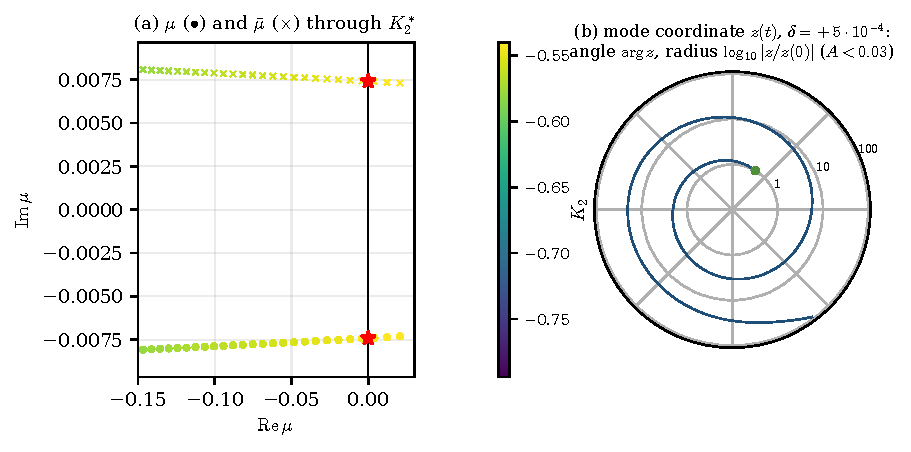
\includegraphics[width=\textwidth]{figures/fig_hopf_orbit.pdf}
\caption{The transverse Hopf point of Theorem~\ref{V3P3:thm:hopf}(a) on $Y_{168}$,
$(K_1,\alpha,\Phi)=(1,0.55,-1.40)$. (a) Along the branch of cluster equilibria, the leading eigenvalue
$\mu$ of the block $M(\lambda)$, $\lambda=2\sqrt2\,e^{-i\varphi}$ (dots), and its conjugate partner
$\bar\mu$ in $M(\bar\lambda)$ (crosses), coloured by $K_2\in[K_2^{*}-0.25,K_2^{*}+0.004]$; they cross the
imaginary axis at $\pm i\Omega_H$, $\Omega_H=0.0074144$ (stars), with speed
$d\operatorname{Re}\mu/dK_2=5.0116$, each with multiplicity $21$. (b) The full $168$-oscillator
network at $K_2=K_2^{*}+5\cdot10^{-4}$, started at amplitude $10^{-4}$ in the $42$-dimensional critical
space: the critical-mode coordinate $z(t)$ in log-polar form (angle $\arg z$, radius
$\log_{10}|z/z(0)|$), shown while the rms deviation $A<0.03$. It turns at the rate $\Omega_H$ and grows at
the linear rate $\operatorname{Re}\mu$ at first, then faster (Remark~\ref{V3P3:rem:hopfdyn}(2)), and
leaves the neighbourhood without settling on a cycle; the trajectory ends in a frequency-locked state.
Drawn by \texttt{code/make\_figures.py}.}
\label{V3P3:fig:hopf}
\end{figure}

\begin{remark}[Numerical: what happens beyond the crossing]\label{V3P3:rem:hopfdyn}
Full-network simulations (RK4, $dt=0.25$) at the point of Theorem~\ref{V3P3:thm:hopf}(a), with
$\delta=K_2-K_2^{*}$:
\begin{enumerate}
\item[(1)] \emph{Linear regime.} For $\delta=+0.0005$ the linearization gives
$\mu=0.00252+0.00740i$. Started at amplitude $10^{-4}$ in the centre space, the rms deviation $A$
grows at rate $0.00255$ and the critical-mode coordinate turns at rate $0.00743$ while
$A\in[2\cdot10^{-4},10^{-3}]$: the instability is the predicted oscillatory one
(Figure~\ref{V3P3:fig:hopf}).
\item[(2)] \emph{No saturation.} The growth then accelerates, to rates $0.0103$ for
$A\in[3\cdot10^{-3},10^{-2}]$ and $0.087$ for $A\in[10^{-2},3\cdot10^{-2}]$: the nonlinearity is
destabilizing, and there is no small-amplitude cycle to land on. The trajectory ends at a state that
is frequency-locked (spread of $\dot\theta_j$ below $2\cdot10^{-13}$) and stationary in the rotating
frame (shape change $4\cdot10^{-16}$), with $A=0.442$ and $r=(0.9994,0.9965,0.8155)$: a relative
equilibrium off the cluster subspace, in which one class is partly desynchronized.
\item[(3)] \emph{All initial directions.} For $\delta=+0.001$ and $+0.002$ (exactly the $42$ Hopf
modes are unstable there), three generic perturbations in the centre space and three pure
character modes (each of the $42$ unstable characters of the deck group spans an invariant
$3$-dimensional subspace) all end in frequency-locked stationary states, with $A$ between $0.40$ and
$0.52$.
\item[(4)] \emph{Below threshold.} The equilibrium is linearly stable, but a perturbation of size
$\varepsilon$ in a fixed generic centre direction escapes to a locked state once
$\varepsilon>\varepsilon_c$, with $\varepsilon_c=0.0053$, $0.0184$, $0.0537$ at $\delta=-0.002$,
$-0.008$, $-0.032$. So $\varepsilon_c\to0$ as $\delta\to0^{-}$, as for a subcritical bifurcation; the
fitted exponent is $0.83$, not the $\frac12$ of a generic cubic normal form, so we do not claim a
normal-form classification.
\item[(5)] \emph{A nearby steady-state crossing.} At every Hopf point examined, a real eigenvalue of
the block of $e^{i\pi/3}$ crosses zero shortly after the Hopf pair: $\delta_{\mathrm{next}}=0.0035$ at
the point of Theorem~\ref{V3P3:thm:hopf}(a), and $0.0005$, $0.0020$, $0.0020$ at three representative
points of (b). This is structural rather than accidental: all blocks share the diagonal $-\sigma_t$, so
when one block reaches the axis the others are close. The transverse Hopf points of $Y_{168}$ thus
sit near a Hopf/steady-state interaction of codimension two.
\item[(6)] \emph{Survey.} At those three representative points, each run at
$\delta=\delta_{\mathrm{next}}/5$ (so that exactly the $42$ Hopf modes are unstable) from a perturbation
of size $10^{-3}$ in the centre space, the outcome is a frequency-locked stationary state in all three
cases ($A=0.27$, $0.22$, $0.32$, each with one class partly desynchronized). An earlier survey of
$12$ Hopf points at $\operatorname{Re}\mu=+0.01$ gave the same outcome in all $12$ cases, with $A$ from
$0.30$ to $1.46$ (at the largest, $r=(0.45,0.45,0.22)$) and $\Omega_H\in[0.0027,0.0076]$.
\item[(7)] \emph{Order parameters.} The critical modes lie in $W_{[\lambda]}\oplus W_{[\bar\lambda]}$,
which is orthogonal to the class indicators (they span $W_{[\kappa]}$, and $A_1$ is normal). So the
class means of the deviation vanish, and $1-r_t=\frac12\operatorname{Var}_{V_t}(\theta)+O(A^{3})$:
the oscillation is visible in $r_0,r_1,r_2$ only at second order, and the time series of the
$r_t$ show the growth (with $1-r_t\propto A^{2}$) and the final jump, not the rotation. The rotation
is seen in the critical-mode coordinate (figure \texttt{v3p3\_hopf\_dynamics.png}).
\end{enumerate}
So transverse Hopf bifurcations exist and account for about a fifth of the losses of stability of
stable cluster states on $Y_{168}$, but no stable limit cycle, chiral or otherwise, was found near
any of them: the loss of stability is hard, and the network freezes into a locked state of the kind
seen in Remark~\ref{V3P3:rem:numerics}(2). This happens even where only the Hopf modes are linearly
unstable, but the nearby steady-state crossing of (5) means that the relevant normal form is that of a
Hopf/steady-state interaction on a $42+7$-dimensional centre space, not of an isolated Hopf point.
Whether some isotropy branch of the equivariant bifurcation is supercritical is open.
\end{remark}

\begin{remark}[Corrections to the proposed programme]\label{V3P3:rem:hopfcorrections}
(1) The crossing is not a simple Hopf bifurcation: on $Y_{168}$ the pair $\pm i\Omega_H$ has
multiplicity $21$ each, forced by the deck-group symmetry (Proposition~\ref{V3P3:prop:hopfstruct}), so
``supercritical'' in the sense of a single first Lyapunov coefficient is not defined. (2) The
bifurcation point $(K_1^{*},K_2^{*},\alpha^{*},\Phi^{*})$ is a curve family, not a point: for fixed
$(\alpha,\Phi)$ there is a value $K_2^{*}$, and Theorem~\ref{V3P3:thm:hopf} gives one to $23$ digits
and the locus at $\alpha=0.55$. (3) Beyond the crossing ($\operatorname{Re}\mu>0$) the simulations do not
produce a stable chiral limit cycle; they produce frequency-locked relative equilibria off the cluster
subspace. (4) The class order parameters $r_t(t)$ see the oscillation only at second order and are
not a good detector of it. (5) The Hopf points are not isolated codimension-one events: a real
crossing in the block of $e^{i\pi/3}$ follows within $\delta_{\mathrm{next}}=0.0005$--$0.0035$.
\end{remark}


\section{Verification battery}\label{V3P3:sec:battery}

\begin{table}[ht]
\centering\scriptsize
\renewcommand{\arraystretch}{1.2}
\resizebox{\textwidth}{!}{%
\begin{tabular}{lcl}
\toprule
check & complexes & result\\
\midrule
(G) $\delta A^{\alpha}=2\pi\alpha$; type gauge shifts $a$ by $2\pi/3$; $H_1(Y_{21})=(\Z/2)^{6}$, $64$ classes & $Y_{21},Y_{24},T_6$ & exact\\
(L) triangle lemma on a $721^{2}$ grid, $200$ values of $S$ & --- & numeric $10^{-4}$\\
(V) twisted state attains $-|E|\cos\frac{2\pi\beta}3$; $30$ random descents never lower & $Y_{21},T_6$ & numeric\\
(J) $J_m=-c_m\Delta_0$, rotation at $K_2\sin\Phi$; the $Y_{21}$ example table & $Y_{21},Y_{24},T_6$ & numeric $10^{-7}$\\
(F) $\frac1n\sum\dot\theta_j=\omega+K_2\langle m_\Delta\rangle_F$ at random states & $Y_{21},Y_{168},T_6$ & numeric $10^{-12}$\\
(R) reduced cluster Jacobian symmetric ($685$ equilibria); field $=-\nabla U+\bar m\mathbf 1$ & --- & numeric\\
(B) spectrum $=\bigcup\operatorname{spec}M(\lambda)\cup\{-\sigma_t\}$ at $46$ equilibria; real on $Y_{21}$; complex on $Y_{168}$ in $6$ & $Y_{21},Y_{168}$ & numeric $10^{-5}$\\
(O) Lyapunov inequality ($2000$ points); $60$ OA runs without chimera limit; OA defect $0.013$ vs $0.36$ & --- & numeric (seeds fixed)\\
(N) $2196$ stable cluster equilibria, none with exactly one stable class; frozen end states; solitary / disordered drift & $Y_{21},Y_{168}$ & numeric (seeds fixed)\\
(E) $\chi=n$ for $q=2$; $\chi(T_6)=0$ & $Y_{21},Y_{24},Y_{168},T_6$ & exact\\
\bottomrule
\end{tabular}}
\medskip
\caption{Checks run by \texttt{code/v3p3\_verify.py}; the complexes are built by
\texttt{code/a2\_common.py}. Section~\ref{V3P3:sec:hopf} is checked by
\texttt{code/v3p3\_hopf\_search.py}.}
\label{V3P3:tab:battery}
\end{table}

\section{Scope, residue, corrections}\label{V3P3:sec:scope}

\begin{remark}[Solved, open]\label{V3P3:rem:scope}
\emph{Solved:} the classification of chiral connections; the gradient structure of the flux
sector, with its frustrated ground states and multistability; the twisted states and their
exact spectra for all parameters; the gradient structure of the cluster subspace; the block
decomposition of the Jacobian at cluster states; OA closure and non-closure; the exclusion of
gauge chimeras for identical oscillators; the frequency sum rule; the monodromy of flux
threading. \emph{Open:}
(a) whether \eqref{V3P3:eq:model} with $K_2\ne0$ has a type-selective chimera on some family
of complexes; transverse Hopf bifurcations through a block $M(\lambda)$ do occur on $Y_{168}$
(Theorem~\ref{V3P3:thm:hopf}), and what remains open is whether any branch of this
multiplicity-$21$ equivariant bifurcation is supercritical (Remark~\ref{V3P3:rem:hopfdyn});
(b) a low-dimensional closure for the triadic term, perhaps for an OA-compatible variant that
is first harmonic in $\theta_j$;
(c) the case $\Delta>0$ of Theorem~\ref{V3P3:thm:nochimera};
(d) the role of the $|H_1|$ flat twists, which break the $\Z/3$ cluster symmetry.
\end{remark}

\begin{remark}[Corrections to the proposed programme]\label{V3P3:rem:corrections}
(1) A nonzero flux does not remove static fixed points or force a limit cycle. For $K_2=0$
the model is a gradient flow for every flux (Theorem~\ref{V3P3:thm:gradient}). Its ground
states are twisted states that carry static persistent currents
(Theorem~\ref{V3P3:thm:ground}). Breaking the conjugation $C$ is not breaking
gradient-ness. (2) $\Phi_\Delta$ is not part of the gauge field. The gauge-covariant triadic
term is blind to the flux (Remark~\ref{V3P3:rem:lag}); the only non-gradient ingredient is
the triadic lag, through the chamber drive (Theorem~\ref{V3P3:thm:clustergrad}). (3) The OA
reduction closes only for $K_2=0$ (Proposition~\ref{V3P3:prop:oa}). (4) There is no Hopf
bifurcation at twisted states, anywhere in the cluster subspace, anywhere for $K_2=0$, or at
any cluster state of $Y_{21}$ (Theorems~\ref{V3P3:thm:twisted}, \ref{V3P3:thm:clustergrad},
\ref{V3P3:thm:gradient}, Corollary~\ref{V3P3:cor:Y21real}). On $Y_{168}$ transverse Hopf points
exist, but they have multiplicity $21$ and, numerically, lead to a hard loss of stability
(Section~\ref{V3P3:sec:hopf}). A supercritical Hopf route to a chimera is not established. (5) The chimera ``$r_0\approx1$, $r_1,r_2$ incoherent'' is
impossible for $K_2=0$ and identical oscillators (Theorem~\ref{V3P3:thm:nochimera}). For
$K_2\ne0$ it is unproved, and it was not seen numerically
(Remark~\ref{V3P3:rem:numerics}). (6) The geometric phase of the synchronized rotation is
$0$. The geometric content is the $\Z/3$ monodromy of flux threading
(Propositions~\ref{V3P3:prop:berry}, \ref{V3P3:prop:monodromy}). (7) $\Delta\Omega=K_2\sin
\Phi$ is local and does not involve $\chi(Y)$ (Theorem~\ref{V3P3:thm:shift},
Remark~\ref{V3P3:rem:euler}). (8) Trees fail because every connection on a tree is pure gauge
and a graph has no $2$-cells, hence no triadic term and no non-gradient dynamics
(Proposition~\ref{V3P3:prop:tree}).
\end{remark}

\section*{Acknowledgement of provenance and caveats}

Unrefereed. The classical inputs are \L{}ojasiewicz's gradient inequality \cite{Loj63} and
LaSalle's invariance principle \cite{LaSalle60}. The Ott--Antonsen ansatz \cite{OA08} is used
only through the computation in Proposition~\ref{V3P3:prop:oa}. The chimera and triadic-coupling
literature \cite{KB02,AMSW08,SK86,SA19} is cited for context and terminology only. The
numerical observations of Remark~\ref{V3P3:rem:numerics} are exploratory and fixed-seed. The
bibliographic data of \cite{Loj63,LaSalle60,OA08,AMSW08,SK86,SA19} have been checked against Crossref and
zbMATH; \cite{KB02}, which neither indexes, was checked against the reference lists of later work.
